
\chapter{How to Visually Communicate}
\label{chpt:visComm}


 Pictures, figures, images, plots, etc. are all forms of visual communication. Any visual communication should be made in the most \textit{effective} and \textit{accessible} way possible. This chapter will discuss what it means to visually communicate effectively and ensure accessibility when creating line and field plots from data. General implementation of these practices in python and MATLAB is provided in Section~\ref{chpt:figCode}. 

\index{plotting}
\index{figure making}

\section{Effective and Accessible Communication}
\label{chpt:effectiveFigs}
Visual communication is effective when the reader immediately understands what is being presented. Labels, such as those in legends and on axes, tell the reader exactly what is presented without the need for assumptions or guessing. Units for the axes set scale which allows the reader to form conclusions of their own without further explanation. Captions describe the visualization in words and include what the reader needs to understand the plot's labels, such as variable definitions. Note that conclusions or analysis \textit{should not} be discussed in captions. Plots can imply if the data is discrete or continuous by using data symbols (scatter plots) or continuous curves (solid lines). Data are generally discrete and should be plotted using symbols, while theory/fits should be plotted as continuous curves. All of these stylistic choices discussed make visual communication more effective.

For visual communication to be completely accessible, no reader should be at a disadvantage due to physical abilities or technological access. Colorblindness can make data difficult to discern if the colors do not contrast, especially when considering those who are completely colorblind or when work is printed in black and white. Efforts to use more than color, such as markers, and to select contrasting colors ensure general readability no matter the case. Assistive technology is capable of converting visual communication to non-visual communication by reading alternative text of images. When publicizing work, it is important to include and use descriptive alternative text so that any visual communication can be understood without seeing the image or figure. 

The next two subsections will discuss class standards for visual communication for line and field plots. Code used to produce plots seen in Figures~\ref{fig:badLines!} and \ref{fig:exampField} is provided in Section~\ref{chpt:figCode}.

\newpage
\subsection{Line Plots}
Consider the presentation of data in Figure~\ref{fig:badLines!}. The figure is arranged in two columns: column (1), on the left, shows a poorly made plot, while column (2), on the right, shows a well-constructed one. The three rows \emph{(a)}, \emph{(b)}, and \emph{(c)} correspond to full RGB color, color as experienced with protanopia (red–green colorblindness), and grayscale, respectively. Table~\ref{tab:lineComparison} compares each flaw of plot (1) with its correction in column (2).


\begin{table}[h!]
    \centering
    \begin{tabular}{|>{\raggedright\arraybackslash}p{3cm}|>{\raggedright\arraybackslash}p{4cm}||>{\raggedright\arraybackslash}p{6cm}|}
        \hline
        \textit{Bad plot traits (seen in 1)} & \textit{Good plot traits \ \ \ \ \ \ \ \  (seen in 2)} & \textit{Impact to reader} \\
        \hline
        No data symbols & Large, differentiable data symbols & Shows where the data actually is. \textbf{Symbols represent data; curves represent theory/fits.} {\small Symbols also keep data distinguishable in the legend and plot when color fails (e.g., poor projector or paper printout).} \\
        Small tick labels (numbers on axes) & Large labels everywhere & \textbf{Make everything larger than you think!} Easier for the viewer to read and interpret the data. \\
        No labels for data, plot, or axes & Fully labeled plot \textbf{with units} & Tells the reader what is being presented and the scale of the problem. \\
        Similar colors for different data & Unique, contrasting colors for each dataset & Keeps data distinguishable for colorblind readers and in grayscale, shown in plots (b) and (c). Similar RGB colors can become identical in both cases. \\
        Linearly scaled axes & Logarithmically scaled axes & Reveals power-law behavior. \\
        No reference lines & Reference lines for $n$-order convergence & Confirms to the reader that the claimed order of convergence is actually achieved. \\
        Programs default font (mismatched with document) & Font matching the document body (e.g., Latin Modern) & Makes plot text consistent with the surrounding \LaTeX{} type, so figures don't look pasted in. \textbf{Computer/Latin Modern or Helvetica/Free Sans are strongly recommended.} \\
        \hline
    \end{tabular}
    \caption{Description of differences in plots shown in Figure~\ref{fig:badLines!} and their impact on readability.}
    \label{tab:lineComparison}
\end{table}


\begin{figure}[!ht]
\begin{framed}
  % ---- Row 1 ----
  \emph{1}(\emph{a})
  \hspace*{7cm}
  \emph{2}(\emph{a})\\
  \hspace*{5mm}
  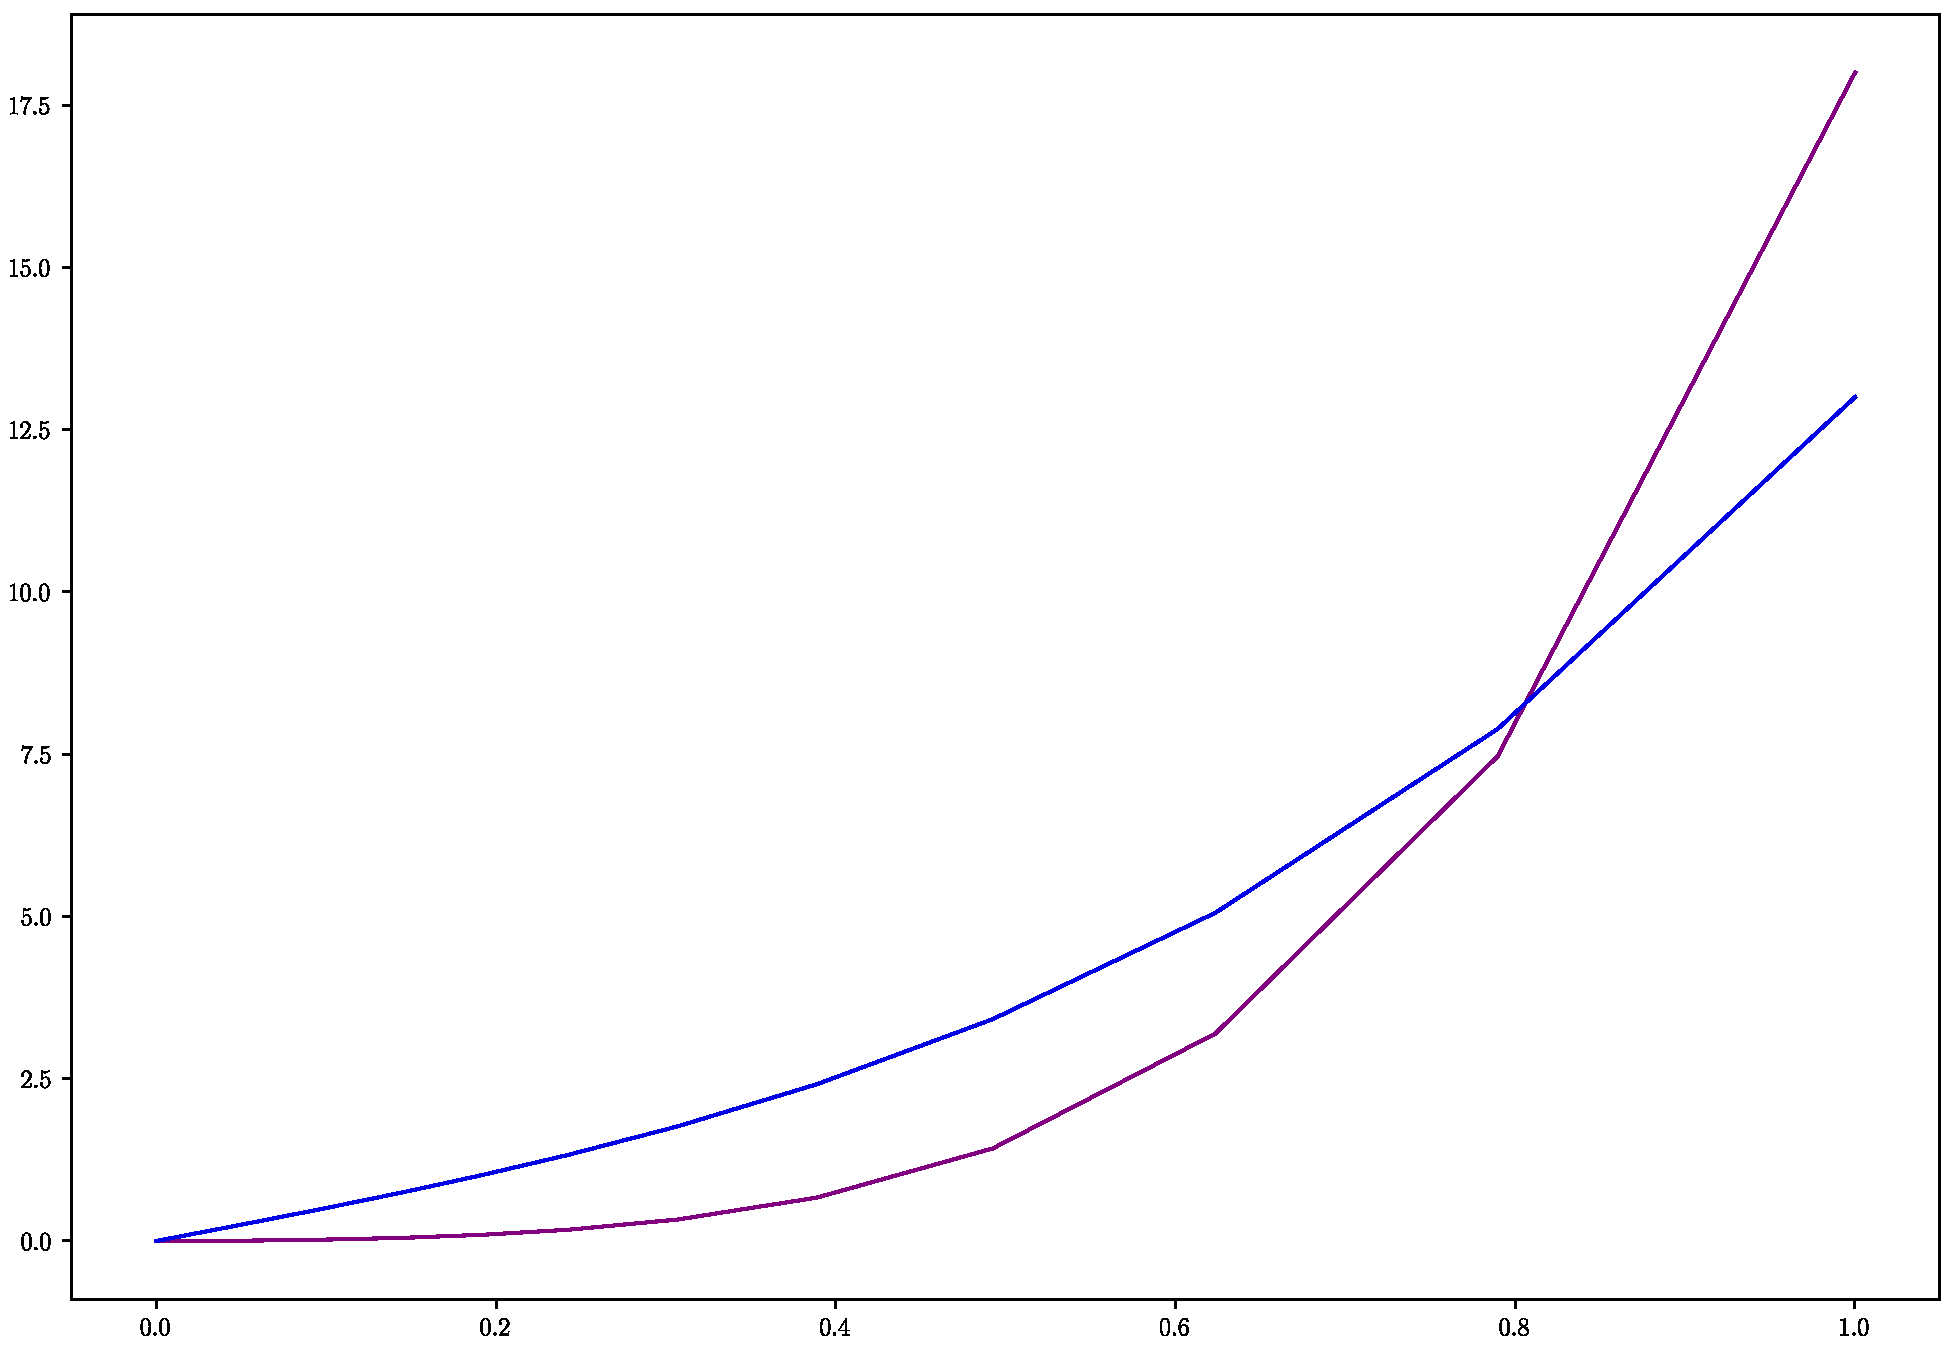
\includegraphics[trim = 0mm 0mm 0mm 0mm,clip,
  width=7.0cm, page=1]{Plots/images/linesv5.pdf}
  \includegraphics[trim = 0mm 0mm 0mm 0mm,clip,
  width=7.0cm, page=4]{Plots/images/linesv5.pdf}\\[2mm]
  % ---- Row 2 ----
  \emph{1}(\emph{b})
  \hspace*{7cm}
  \emph{2}(\emph{b})\\
  \hspace*{5mm}
  \includegraphics[trim = 0mm 0mm 0mm 0mm,clip,
  width=7.0cm, page=2]{Plots/images/linesv5.pdf}
  \includegraphics[trim = 0mm 0mm 0mm 0mm,clip,
  width=7.0cm, page=5]{Plots/images/linesv5.pdf}\\[2mm]
  % ---- Row 3 ----
  \emph{1}(\emph{c})
  \hspace*{7cm}
  \emph{2}(\emph{c})\\
  \hspace*{5mm}
  \includegraphics[trim = 0mm 0mm 0mm 0mm,clip,
  width=7.0cm, page=3]{Plots/images/linesv5.pdf}
  \includegraphics[trim = 0mm 0mm 0mm 0mm,clip,
  width=7.0cm, page=6]{Plots/images/linesv5.pdf}\\[2mm]
  \caption{Column 1 and Column 2 represent line plots of the same dataset with different plotting styles. The three rows \emph{(a)}, \emph{(b)}, and \emph{(c)} correspond to full RGB color, color as experienced with protanopia (red–green colorblindness), and grayscale, respectively.}
  \label{fig:badLines!}
  \vspace*{2mm}
\end{framed}
\end{figure}




% The second row showcases the same data presented in an effective and accessible way. The data is properly labeled, concisely describing the type of data and the different lines being presented. The addition of the star and circle marker makes the plot accessible when color is not available. Figure~\ref{fig:badLines!}\emph{(c)} showcases the same colors as \emph{(a)} for the respective curves but mimics protanopia (red-green colorblindness), highlighting the need to select colors that are distinct and contrasting. Increasing the linewidth of plotted curves, axes, and legend boxes effectively contrasts the information with the white background and stands out to the reader. Notice the font now matches standard \LaTeX, ensuring typeset continuity throughout the document.





% \begin{figure}[!ht]
% \begin{framed}
%   % ---- Row 1 ----
%   (\emph{a})
%   \hspace*{7cm}
%   (\emph{b})\\
%   \hspace*{5mm}
%   \includegraphics[trim = 0mm 0mm 0mm 0mm,clip,
%   width=7.0cm, page=4]{Plots/images/fields.pdf}
%   \includegraphics[trim = 0mm 0mm 0mm 0mm,clip,
%   width=7.0cm, page=6]{Plots/images/fields.pdf}\\[2mm]
%   % ---- Row 2 ----
%   (\emph{c})
%   \hspace*{7cm}
%   (\emph{d})\\
%   \hspace*{5mm}
%   \includegraphics[trim = 0mm 0mm 0mm 0mm,clip,
%   width=7.0cm, page=2]{Plots/images/fields.pdf}
%   \includegraphics[trim = 0mm 0mm 0mm 0mm,clip,
%   width=7.0cm, page=3]{Plots/images/fields.pdf}\\[-7mm]
%     % ---- Row 3 ----
%   (\emph{c})
%   \hspace*{7cm}
%   (\emph{d})\\
%   \hspace*{5mm}
%   \includegraphics[trim = 0mm 0mm 0mm 0mm,clip,
%   width=7.0cm, page=2]{Plots/images/fields.pdf}
%   \includegraphics[trim = 0mm 0mm 0mm fields,clip,
%   width=7.0cm, page=3]{Plots/images/lines.pdf}\\[-7mm]
%   \caption{Three rows of some field, where each row represents a different colormap and each column represents different views of color. Row }
%   \label{fig:badLines!}
%   \vspace*{2mm}
% \end{framed}
% \end{figure}

\clearpage 
\newpage
\subsection{Field Plots}


Plotting fields is an effective way to understand what a system is doing at an instance of time.  Efforts to make fields more effective and accessible are focused on ensuring the labels are clear and a good colormap is selected. 

\begin{figure}[!ht]
    \centering
    
\includegraphics[width=0.75\linewidth]{Plots/images/blues.jpg}\\ [4mm]
    % \hspace{6cm}
    % \vspace{1cm}
    
\includegraphics[width=0.75\linewidth]{Plots/images/curl.jpg}
    \caption{A sequential colormap (\textit{blues}) on top and a diverging colormap (\textit{curl}) on bottom. Colormaps from \textcite{cmapRepo}.}
    \label{fig:turboCM}
\end{figure}

A colormap is a gradient of color, as seen in Figure~\ref{fig:turboCM}. Colormaps map numerical values of a field to colors along its gradient, which lets us visualize how the field changes across space and time. Different styles of colormap suit different applications; here we consider \textit{sequential} and \textit{divergent} maps.


Sequential colormaps change monotonically from one end to the other, like the \textit{blues} map at the top of Figure~\ref{fig:turboCM} which runs from a dark color to a bright one. These maps are effective for fields where it is important to see growth or subtle changes in magnitude across the field.

Divergent colormaps change monotonically from each end toward the middle, where two dark colors meet at a bright center — as in the \textit{curl} map from cmocean \parencite{cmoceanRep} shown at the bottom of Figure~\ref{fig:turboCM}. They are effective for fields centered around some mean value since they highlight variation away from that center and make the largest deviations stand out.




\begin{figure}[!ht]
\begin{framed}
  % ---- Row 1 ----
  \emph{1}(\emph{a})
  \hspace*{7cm}
  \emph{2}(\emph{a})\\
  \hspace*{5mm}
  \includegraphics[trim = 0mm 0mm 0mm 0mm,clip,
  width=7.0cm]{Plots/images/compCMAPSeqFlat.pdf}
  \includegraphics[trim = 0mm 0mm 0mm 0mm,clip,
  width=7.0cm]{Plots/images/compCMAPDivFlat.pdf}\\[2mm]
  % ---- Row 2 ----
  \emph{1}(\emph{b})
  \hspace*{7cm}
  \emph{2}(\emph{b})\\
  \hspace*{5mm}
  \includegraphics[trim = 4mm 4mm 4mm 4mm,clip,
  width=7.0cm, page=2]{Plots/images/compCMAP3D.pdf}
  \includegraphics[trim = 4mm 4mm 4mm 4mm,clip,
  width=7.0cm, page=1]{Plots/images/compCMAP3D.pdf}\\[2mm]
  \caption{Column 1 and Column 2 represent field plots of the same dataset with different plotting styles. The two rows \emph{(a)} and \emph{(b)} correspond to flat pseudocolor plots and 3D plots, respectively.}
  \label{fig:exampleFields}
  \vspace*{2mm}
\end{framed}
\end{figure}




%When $t=0$, a drop fell in the center, sending waves of a circular pattern away from the point of impact. 



Consider the two-dimensional fields shown in Figure~\ref{fig:exampleFields}. The field in column 1 is considered sequential, as the data grows monotonically to peaks across the field. The field is column two is divergent, with discontinuous oscillations about $f(x,y) = 0$. A divergent color map clearly shows where these oscillations are, and the general pattern they have across the field. This pattern is much more apparent in the two-dimensional (2D) plot (2b), where as the three-dimensional (3D) plot (2b) does not accurately reflect the field, as much of the field at the center is hidden by the large magnitude oscillations along the $x$ axis. When plotting in 3D, it is important to consider the angle at which the data is plot, as the surface can hid information when certain angles are chosen. Generally, it is the best choice to plot in 2D.



% What then makes a good colormap and are there standard choices that are both effective and accessible? To answer this, we consider Figure~\ref{fig:fieldsPlots}, which showcases three colormaps as respective rows in both full color (column one) and grayscale (column two). We will discuss \textit{ice}, \textit{jet}, and \textit{turbo}.



\clearpage 
\clearpage
\begin{figure}[!ht]
\begin{framed}
\centering
\setlength{\tabcolsep}{2pt}
\begin{tabular}{c c}
  % ---- Row 1 ----
  \rotatebox{90}{\makebox[6cm][c]{\emph{Row 1: full RGB}}}
  & 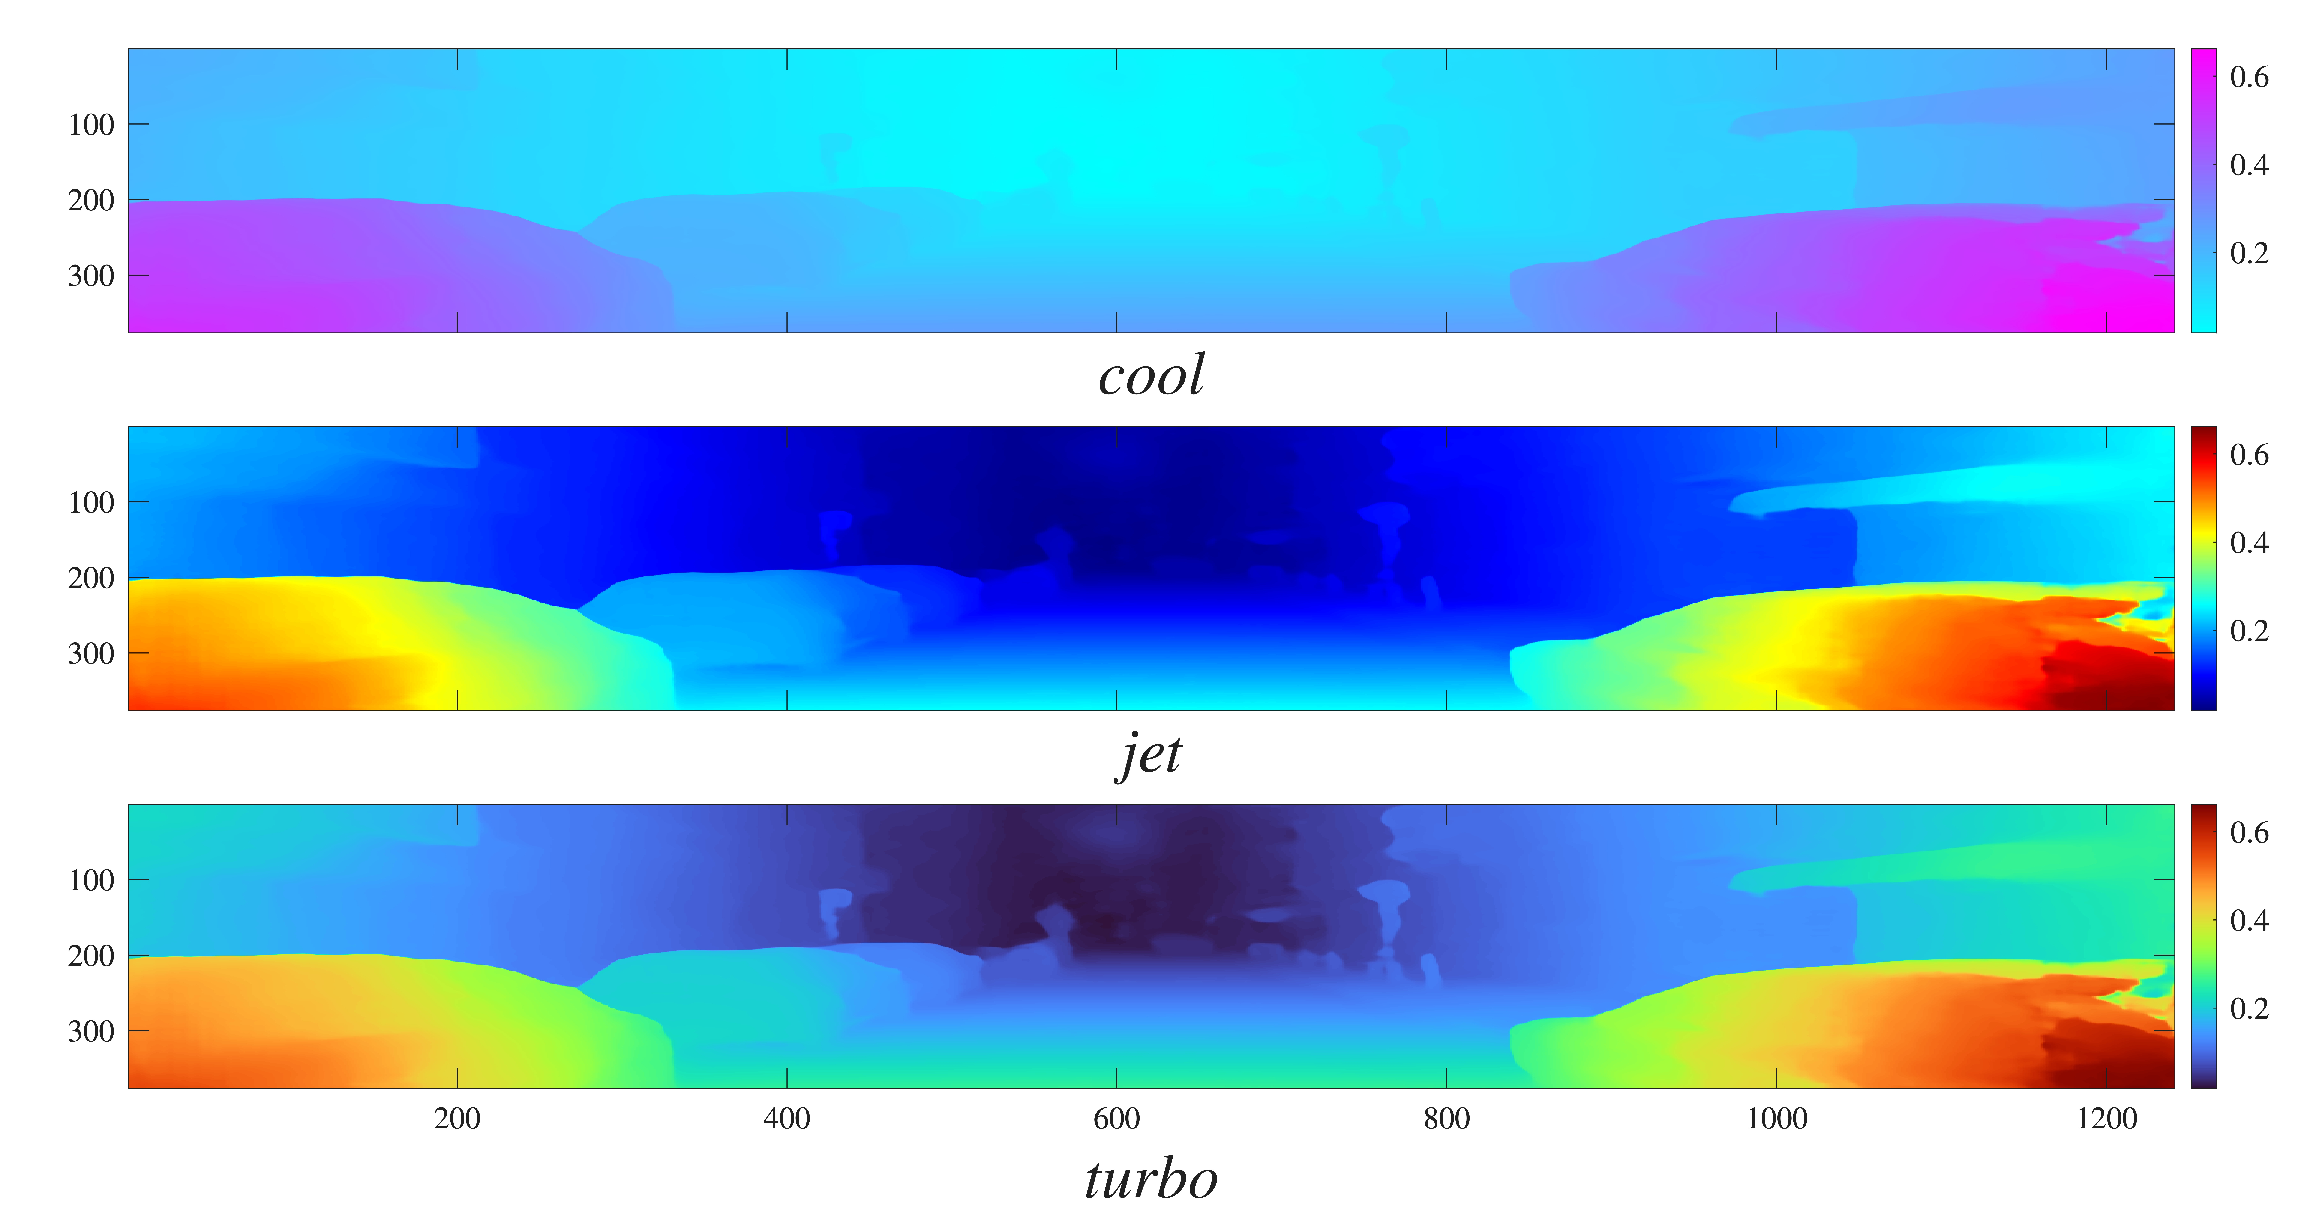
\includegraphics[width=0.80\linewidth]{Plots/images/dispRBG.pdf} \\
  % ---- Row 2 ----
  \rotatebox{90}{\makebox[6cm][c]{\emph{Row 2: colorblind}}}
  & 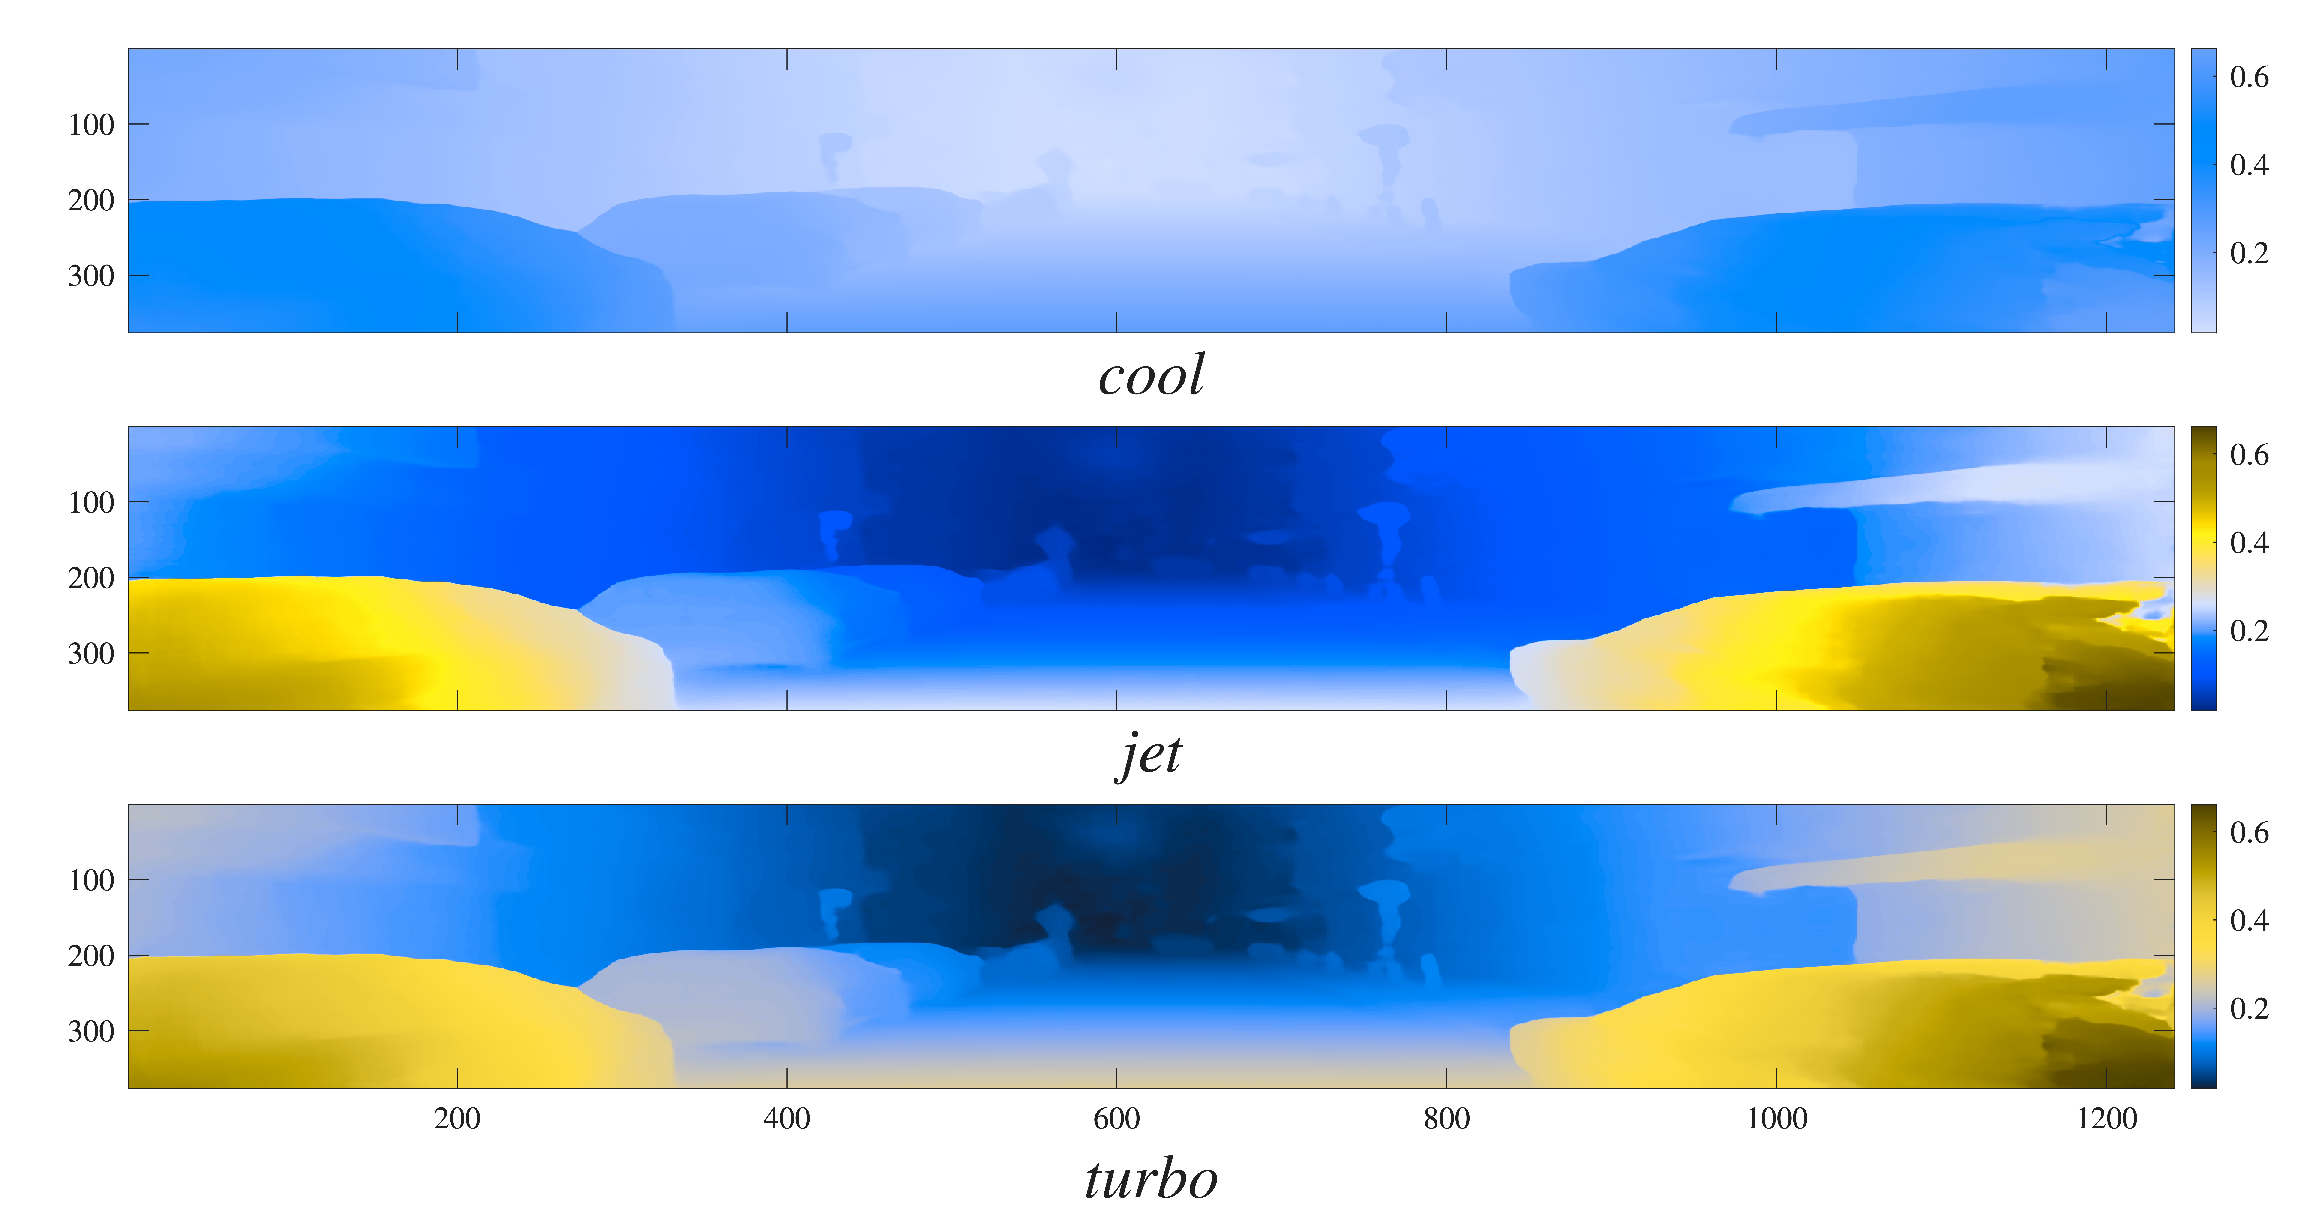
\includegraphics[width=0.80\linewidth]{Plots/images/dispProton.pdf} \\
  % ---- Row 3 ----
  \rotatebox{90}{\makebox[6cm][c]{\emph{Row 3: grayscale}}}
  & 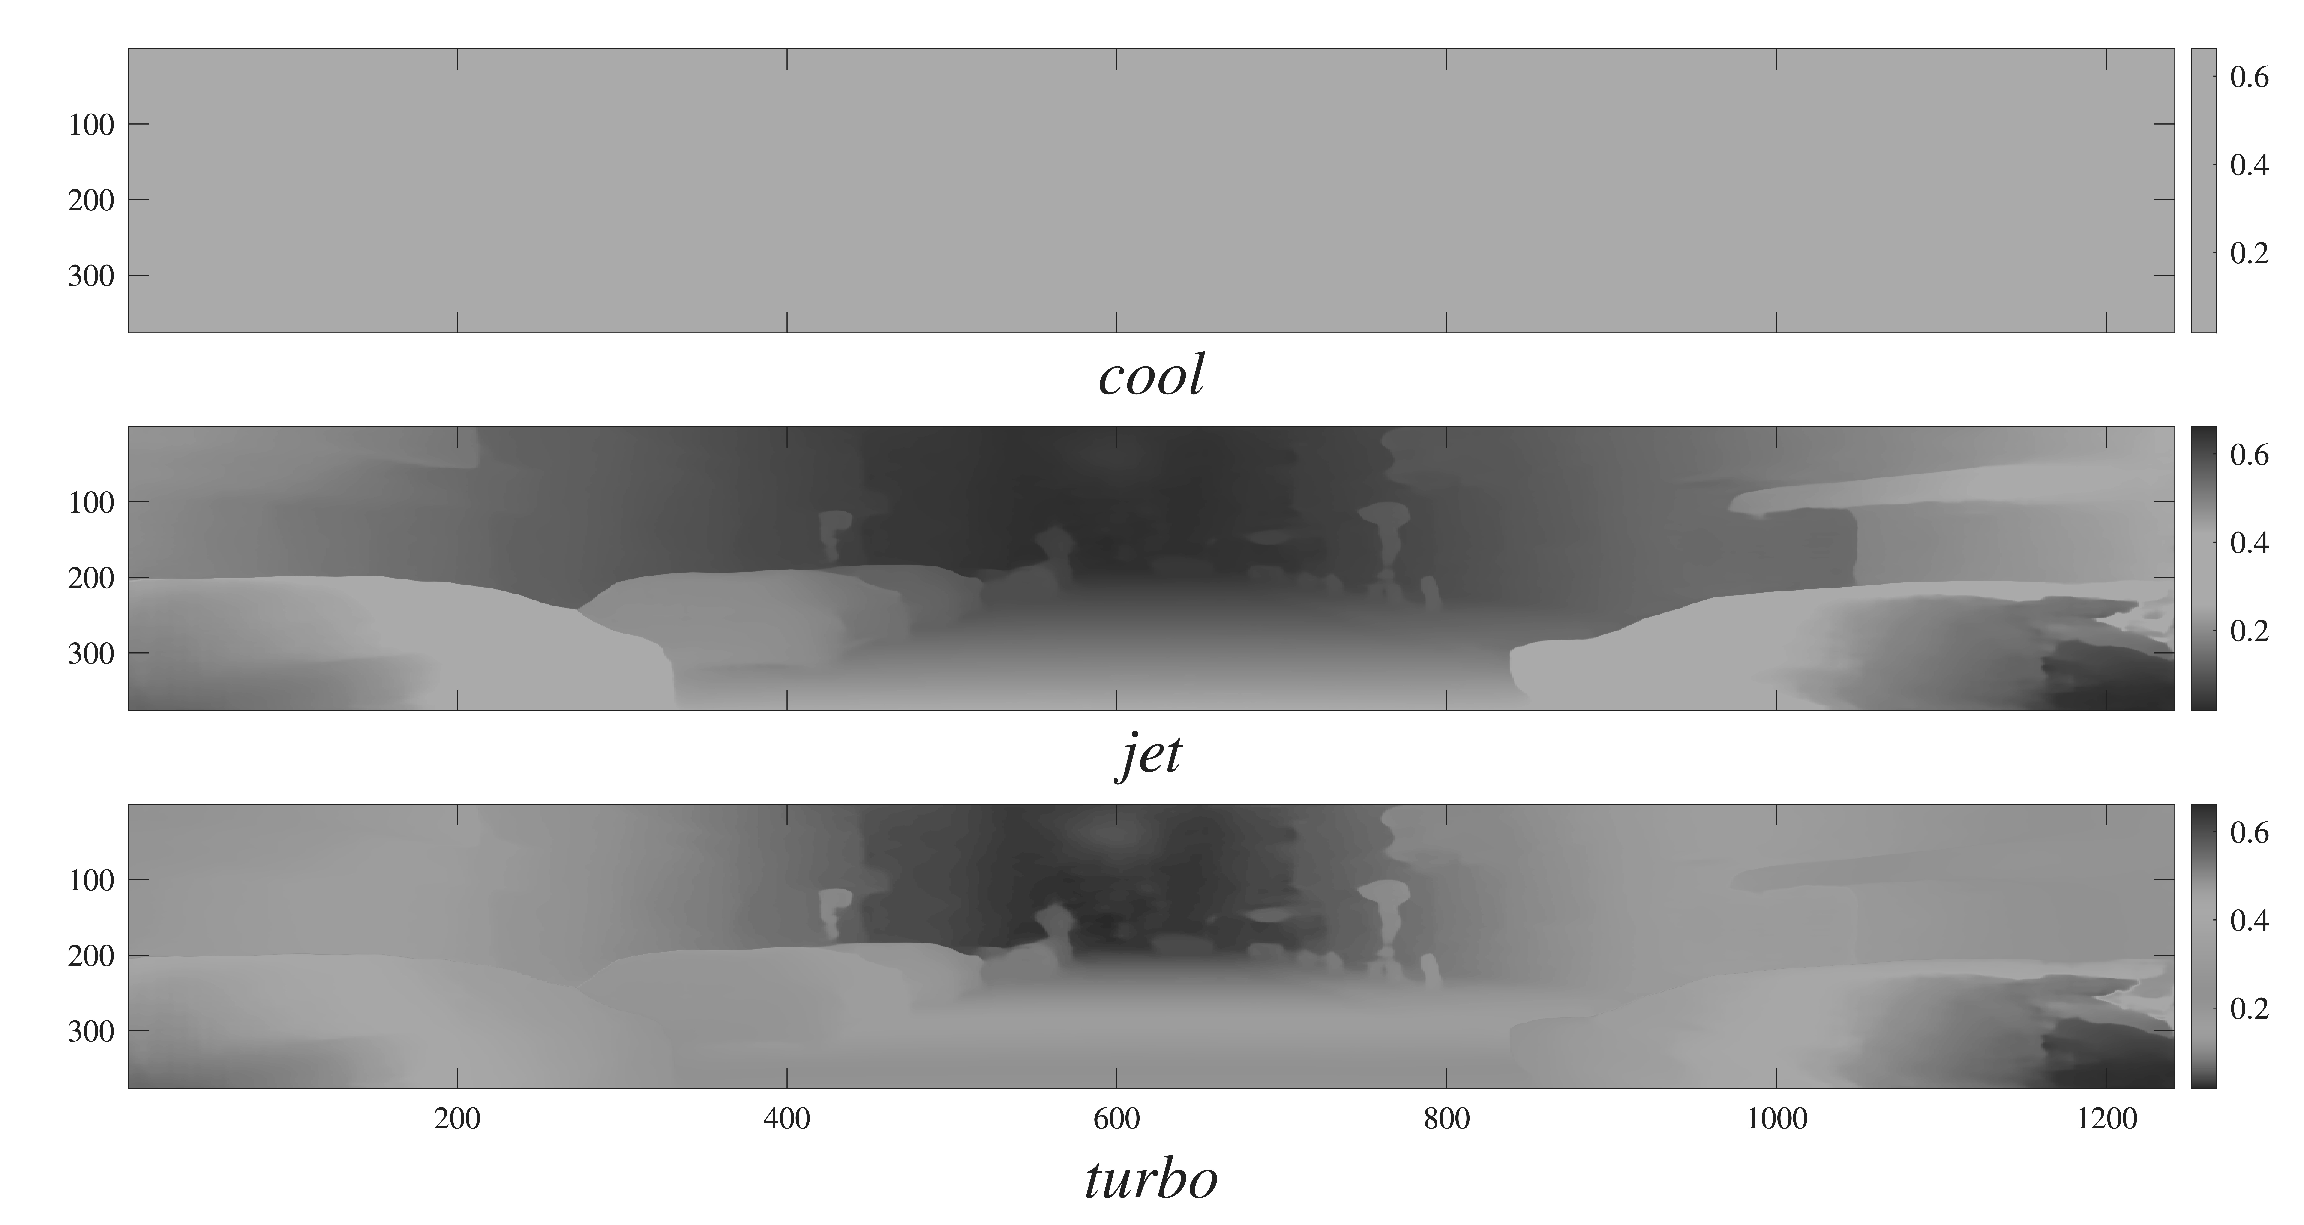
\includegraphics[width=0.80\linewidth]{Plots/images/dispMono.pdf} \\
\end{tabular}
\caption{wip}
\label{fig:fieldsPlots}
\end{framed}
\end{figure}

% { \Large \textcolor{magenta}{fix caption and once thats decided make as big as possible ALSO READ THRU CODE TO QC} }

\clearpage

% Now, let's consider . Each row of showcases the same data as that in  Figure~\ref{fig:exampField}, but with different colormaps. When choosing colormaps, it is important to consider both what is being presented and if the map is accessible. You may be drawn to the \textit{ice} colormap shown in row 1, as blue is a natural color choice for fluid or you enjoy it. However, \textit{ice} in grayscale washes out the gradient between the rings of "waves", making the field look more binary than connected. Row 2 shows \textit{jet}, once a quite popular colormap. You'll   

\section{Implementations}
\label{chpt:figCode}

{
\centering
\subsubsection{Lines in python}
\hrule{}
}

\begin{lstlisting}[language=python]
# plotting package import
import matplotlib.pyplot as plt
# numerics package import
import numpy as np

# LaTeX rendering in Latin Modern
plt.rcParams['text.usetex'] = True
plt.rcParams['text.latex.preamble'] = r'\usepackage{lmodern}'
plt.rcParams['font.family'] = 'serif'

# generate data
dxs = np.logspace(-4, 0, 40)  # grid spacings, 10^-4 to 10^0
y1 = 5.0*(dxs) + 8.0*(dxs**3)     # first order error curve
y2 = 2.0*(dxs**2) + 16.0*(dxs**4) # second order error curve

# reference lines (order one ref. is just dxs itself)
ref2 = dxs**2  # order two reference line

fs = 50  # set font size variable

# this is how you define non-standard colors! 
# all these values are the RBG #/255. this accepts both the 
# calculation (67/255) and the fraction (0.2627) for RBG triplets (see below)
badCols = np.array([
    [0.5, 0.000, 0.5],  # purple
    [0, 0, 0.9],        # blue
])


cols = np.array([
    [67/255, 179/255, 174/255],   # teal (marker edge/line 1)
    [136/255, 216/255, 192/255],  # light green (marker face 1)
    [198/255, 97/255, 166/255],   # light magenta (marker face 2)
    [202/255, 44/255, 146/255],   # magenta (marker edge/line 2)
])

# define figure, axes, and size
fig, ax = plt.subplots(figsize=(13, 9))

# bad color choice example (uses badCols)
# ax.plot(dxs, y1, '-', color=badCols[0, :])
# ax.plot(dxs, y2, '-', color=badCols[1, :])

# reference lines (excluded from legend)
ax.plot(dxs[:20], dxs[:20], '-.', color='black',
        linewidth=5, 
        label='_nolegend_') # this excludes this line from the legend
ax.plot(dxs[:20], 0.3*ref2[:20], '--', color='black',
        linewidth=5, label='_nolegend_')

# plots y1 vs dxs every third point as solid line with markers
ax.plot(dxs[::3], y1[::3], '-o',
        color=cols[0, :],            # set line color
        linewidth=2,                 # set line width
        markersize=24,               # set marker size
        markeredgewidth=3,           # set marker outline width
        markeredgecolor=cols[0, :],  # set marker outline color
        markerfacecolor=cols[1, :],  # set marker fill color
        label='first order')         # set legend entry

ax.plot(dxs[::3], y2[::3], '-*', color=cols[3, :], linewidth=2,
        markersize=40, markeredgewidth=3, markeredgecolor=cols[3, :],
        markerfacecolor=cols[2, :], label='second order')

# label reference slopes directly on the plot
ax.annotate(r'$\mathcal{O}(\Delta x)$',
            (1.3*dxs[5], 0.3*dxs[5]), fontsize=0.75*fs)
ax.annotate(r'$\mathcal{O}(\Delta x^2)$',
            (2.3*dxs[5], 0.4*(dxs[5]**2)), fontsize=0.75*fs)

# the multiplications you see above are simply translating the position to get 
# the labels off the line but close to it!

for spine in ax.spines.values():  # set axes line width
    spine.set_linewidth(3)
ax.tick_params(width=3, labelsize=fs)  # set tick width and font size
ax.tick_params(axis='x', pad=10)       # pad ticks away from axis (preventing overlap)

ax.set_xlabel(r'$\Delta x$  (mm)', fontsize=fs, labelpad=2)
ax.set_ylabel(r'Error', fontsize=fs)

ax.legend(fontsize=0.75*fs, loc='lower right')
ax.set_title('Convergence Plot', fontsize=fs)

# set the axis scale to log log
ax.set_xscale('log')
ax.set_yscale('log')
ax.grid() # sets major grid lines - can have settings here

# plt.show()  # uncomment to view interactively

## note: fig will not save if plt.show() is before plt.savefig(...)!!!!
# plt.savefig("linePlotExample.pdf", dpi=800)  # uncomment to export figure (dpi sets raster resolution)
\end{lstlisting}

{
\centering
\subsubsection{Fields in python}
\hrule
}

 \begin{lstlisting}[language=python]
# plotting package import
import matplotlib.pyplot as plt
# numerics package import
import numpy as np

# LaTeX rendering in Latin Modern
plt.rcParams['text.usetex'] = True
plt.rcParams['text.latex.preamble'] = r'\usepackage{lmodern}'
plt.rcParams['font.family'] = 'serif'

# generate data
dx = 0.01
x = np.arange(-np.pi, np.pi + dx, dx)  # + dx includes endpoint
y = x
X, Y = np.meshgrid(x, y) # creates mesh of x and y (2D fields)

# diverging colormap example (use cmap='PiYG' in pcolormesh)
###########################################################
R = np.sqrt(X**2 + Y**2)
f = Y * np.sin(2.0 * R**2)
###########################################################

# sequential colormap example (use cmap='Blues' in pcolormesh)
###########################################################
# f = R * 1.3**(1.01*(abs(abs(X)*abs(Y) - 2*np.pi)) + np.pi/2)
###########################################################

fs = 35  # set font size variable

fig, ax = plt.subplots(figsize=(12, 9))  # set figure size

ax.set_aspect('equal')  # force square aspect ratio

# pseudocolor plot of f across X and Y
# gouraud shading interpolates between cells (no mesh lines)
pc = ax.pcolormesh(X, Y, f, cmap='PiYG', shading='gouraud')

ax.set_xlabel('$x$', fontsize=fs)  # label x-axis in latex
ax.set_ylabel('$y$', fontsize=fs)  # label y-axis in latex

for spine in ax.spines.values():  # set axes line width
    spine.set_linewidth(3)
ax.tick_params(width=3, labelsize=fs)  # set tick width and font size

axesLims = [-np.pi, np.pi]  # define axes limits
ax.set_xlim(axesLims)       # set x axis limits
ax.set_ylim(axesLims)       # set y axis limits

cb = fig.colorbar(pc, ax=ax)                  # add colorbar
cb.ax.tick_params(labelsize=fs)               # set colorbar tick size
cb.set_label('Field Magnitude', fontsize=fs)  # label colorbar

# tick locations and latex labels
ticks = [-np.pi, -np.pi/2, 0, np.pi/2, np.pi]
tickLabel = ['$-\\pi$', '$-\\pi/2$', '$0$', '$\\pi/2$', '$\\pi$']

ax.set_xticks(ticks)           # set x tick locations
ax.set_yticks(ticks)           # set y tick locations
ax.set_xticklabels(tickLabel)  # set x tick labels to tex strings
ax.set_yticklabels(tickLabel)  # set y tick labels to tex strings

# plt.show()  # uncomment to view interactively

## note: fig will not save if plt.show() is before plt.savefig(...)!!!!
# plt.savefig("divergencePlotExample.pdf", dpi=800)  # uncomment to export figure 
# (dpi sets raster resolution)

#### 3D Plot

fig, ax = plt.subplots(subplot_kw={"projection": "3d"}, figsize=(12,9))

ax.plot_surface(X, Y, f, cmap=cm)

fs = 0.8*fs


ticks = [-np.pi, -np.pi/2, 0, np.pi/2, np.pi]  # defining location of ticks
tickLabel = ['$-\\pi$', '$-\\pi/2$', '$0$', '$\\pi/2$', '$\\pi$']  # defining labels for ticks

ax.set_xticks(ticks)            # set x ticks to ticks array
ax.set_yticks(ticks)            # set y ticks to ticks array
ax.set_xticklabels(tickLabel)   # set labels to tex strings in tickLabel
ax.set_yticklabels(tickLabel)   # set labels to tex strings in tickLabel


ax.set_xlabel('$x$', fontsize=fs, labelpad=20)  # label x-axis as x in latex
ax.set_ylabel('$y$', fontsize=fs, labelpad=20)
ax.set_ylabel('$f(x,y)$', fontsize=fs, labelpad=20)

for spine in ax.spines.values():   # set axes linewidth
    spine.set_linewidth(3)
ax.tick_params(width=3, labelsize=fs)  # set tick width and font size

axesLims = [-np.pi - 0.3, np.pi + 0.3]  # define axes limits
ax.set_xlim(axesLims)       # set x axis limits
ax.set_ylim(axesLims)       # set y axis limits

plt.show()

# plt.savefig("seq3D.pdf", dpi=800)
\end{lstlisting}


{
\centering
\subsubsection{Lines in MATLAB}
\hrule
}

 \begin{lstlisting}[language=matlab]

% generate data
dxs = logspace(-4, 0, 40);         % grid spacings, 10^-4 to 10^0

y1 = 5.0*dxs + 8.0*dxs.^3;         % first order error curve
y2 = 2.0*dxs.^2 + 16.0*dxs.^4;     % second order error curve

% reference lines (order one ref. is just dxs itself)
ref2 = dxs.^2;  % order two reference line

fs = 50;  % set font size variable

% rgb colors, defined 0-1
badCols = [0.5 0.0 0.5;    % purple
           0.0 0.0 0.9];   % blue

cols = [ 67 179 174;   % teal (marker edge/line 1)
        136 216 192;   % light green (marker face 1)
        198  97 166;   % light magenta (marker face 2)
        202  44 146] / 255;  % magenta (marker edge/line 2)

% define figure, axes, and size
fig = figure( ...
    "Theme", "light", ...               % plot light even in dark mode
    'Position', [100, 100, 1300, 900]); % match figsize(13,9)

hold on  % ensures all following plot commands go onto fig

% bad color choice example (uses badCols)
% plot(dxs, y1, '-', 'Color', badCols(1,:))
% plot(dxs, y2, '-', 'Color', badCols(2,:))

% reference lines (excluded from legend, truncated to lower half)
plot(dxs(1:20), dxs(1:20), '-.', 'Color', 'black', ...
    'LineWidth', 5, 'HandleVisibility', 'off')
plot(dxs(1:20), 0.3*ref2(1:20), '--', 'Color', 'black', ...
    'LineWidth', 5, 'HandleVisibility', 'off')

% plots y1 vs dxs every third point as solid line with markers
plot(dxs(1:3:end), y1(1:3:end), '-o', ...
    'Color', cols(1,:), ...            % set line color
    'LineWidth', 2, ...                % set line width
    'MarkerSize', 24, ...              % set marker size
    'MarkerEdgeColor', cols(1,:), ...  % set marker outline color
    'MarkerFaceColor', cols(2,:), ...  % set marker fill color
    'DisplayName', 'first order')      % set legend entry

plot(dxs(1:3:end), y2(1:3:end), '-p', 'Color', cols(4,:), ...
    'LineWidth', 2, 'MarkerSize', 40, ...
    'MarkerEdgeColor', cols(4,:), 'MarkerFaceColor', cols(3,:), ...
    'DisplayName', 'second order')

% label reference slopes directly on the plot
text(1.3*dxs(6), 0.3*dxs(6), '$$\mathcal{O}(\Delta x)$$', ...
    'Interpreter', 'latex', 'FontSize', 0.75*fs)
text(2.3*dxs(6), 0.4*dxs(6)^2, '$$\mathcal{O}(\Delta x^2)$$', ...
    'Interpreter', 'latex', 'FontSize', 0.75*fs)

ax = gca;  % pull the current axes
set(ax, ...
    'XScale', 'log', ...              % set x-scale to log
    'YScale', 'log', ...              % set y-scale to log
    'LineWidth', 3, ...               % set axes line width
    'FontSize', fs, ...               % set tick font size
    'TickLabelInterpreter', 'latex'); % set tick interpreter to latex

grid on  % turn on major grid

xlabel('$$\Delta x$$  (mm)', ...  % label x-axis in latex
    'Interpreter', 'latex', ...   % interpret label with latex
    'FontSize', fs);              % set font size of label

ylabel('Error', 'Interpreter', 'latex', 'FontSize', fs);

legend('FontSize', 0.75*fs, ...   % set legend font size
    'Location', 'southeast', ...  % legend bottom right
    'Interpreter', 'latex');      % interpret with latex

title('Convergence Plot', ...    % set plot title
    'Interpreter', 'latex', ...  % interpret title in latex
    'FontSize', fs);             % set font size of title

hold off

saveas(fig, 'convergencePlot.pdf')  % export figure as a pdf




\end{lstlisting}

{
\centering
\subsubsection{Fields in MATLAB}
\hrule
}
 \begin{lstlisting}[language=matlab]

% point matlab to any cmap directories you download
% needed for curl and blues
addpath('<path to directory>/cmap/')

cm = curl(256);

% generate data
dx = 0.01;
x = -pi:dx:pi;
y = x;
[X, Y] = meshgrid(x, y);  % creates mesh of x and y (2D fields)

% diverging colormap example (use colormap('curl'))
%%%%%%%%%%%%%%%%%%%%%%%%%%%%%
R = sqrt(X.^2 + Y.^2);
f = Y.*sin(2.0*R.^2);
%%%%%%%%%%%%%%%%%%%%%%%%%%%%%

% sequential colormap example (use colormap('Blues'))
%%%%%%%%%%%%%%%%%%%%%%%%%%%%%
% f = R .* 1.3.^(1.01*(abs(abs(X).*abs(Y) - 2*pi)) + pi/2);
%%%%%%%%%%%%%%%%%%%%%%%%%%%%%

 % set colormap to match the example above

fs = 35;  % set font size variable

fig = figure( ...
    "Theme", "light", ...               % plot light even in dark mode
    'Position', [100, 100, 1200, 900]); % match figsize(12,9)

hold on  % ensures all following plot commands go onto fig

daspect([1 1 1])  % force square aspect ratio

% pseudocolor plot of f across X and Y
pc = pcolor(X, Y, f);
colormap(cm);
shading interp     % interpolate between cells (matches gouraud)


xlabel('$$x$$', ...              % label x-axis in latex
    'Interpreter', 'latex', ...  % interpret label with latex
    'FontSize', fs);             % set font size of label

ylabel('$$y$$', 'Interpreter', 'latex', 'FontSize', fs);

ax = gca;  % pull the current axes
set(ax, 'LineWidth', 3, 'FontSize', fs)  % set axes width, font size

axesLims = [-pi, pi];  % define axes limits
xlim(axesLims)         % set x axis limits
ylim(axesLims)         % set y axis limits

cb = colorbar('TickLabelInterpreter', 'latex', ...  % add colorbar
    'FontSize', fs);                                % set tick size
ylabel(cb, 'Field Magnitude', ...  % label colorbar
    'FontSize', fs, ...            % set font size
    'Interpreter', 'latex');       % set label interpreter

% tick locations and latex labels
ticks = [-pi, -pi/2, 0, pi/2, pi];
tickLabel = {'$$-\pi$$', '$$-\pi/2$$', '$$0$$', ...
             '$$\pi/2$$', '$$\pi$$'};

ax.TickLabelInterpreter = 'latex';  % set tick interpreter to latex
ax.XTick = ticks;                   % set x tick locations
ax.YTick = ticks;                   % set y tick locations
ax.XTickLabel = tickLabel;          % set x tick labels to tex strings
ax.YTickLabel = tickLabel;          % set y tick labels to tex strings

hold off

%% note: exports whatever figure is current!
% exportgraphics(fig, 'div.pdf', 'Resolution', 800)

%%---------------------------
%% 3D PLOT
%%---------------------------

fig = figure( ...
    "Theme", "light", ...               % plot light even in dark mode
    'Position', [100, 100, 1200, 900]); % match figsize(12,9)

% surface plot of f across X and Y
s = surf(X, Y, f, 'EdgeColor', 'none'); % EdgeColor none removes mesh lines
colormap(cm);  % set colormap (cm defined above)

fs = 0.8*fs;  % shrink fonts for the 3d view

% tick locations and latex labels
ticks = [-pi, -pi/2, 0, pi/2, pi];
tickLabel = {'$$-\pi$$', '$$-\pi/2$$', '$$0$$', ...
             '$$\pi/2$$', '$$\pi$$'};

ax = gca;  % pull the current axes
ax.TickLabelInterpreter = 'latex';  % set tick interpreter to latex
ax.XTick = ticks;                   % set x tick locations
ax.YTick = ticks;                   % set y tick locations
ax.XTickLabel = tickLabel;          % set x tick labels to tex strings
ax.YTickLabel = tickLabel;          % set y tick labels to tex strings

xlabel('$$x$$', ...              % label x-axis in latex
    'Interpreter', 'latex', ...  % interpret label with latex
    'FontSize', fs);             % set font size of label

ylabel('$$y$$', 'Interpreter', 'latex', 'FontSize', fs);
zlabel('$$f(x,y)$$', 'Interpreter', 'latex', 'FontSize', fs);

set(ax, 'LineWidth', 3, 'FontSize', fs)  % set axes width, font size

axesLims = [-pi - 0.3, pi + 0.3];  % define axes limits (small margin)
xlim(axesLims)                     % set x axis limits
ylim(axesLims)                     % set y axis limits

%% note: exports whatever figure is current!
% exportgraphics(fig, 'seq3D.pdf', 'Resolution', 800)

\end{lstlisting}





% \begin{wrapfigure}{r}{6.2cm}
%   \vspace*{-0.7cm}
% \begin{framed}

%   % (\emph{a})
%   % \hspace*{3cm}
%   % (\emph{b})\\[1mm]
%   % \hspace*{-4mm}
%   \includegraphics[trim = 0mm 0mm 0mm 0mm,clip,width=5.5cm, page=2]{Plots/images/compCMAP.pdf}
%     \includegraphics[trim = 0mm 0mm 0mm 0mm,clip,width=5.5cm, page=1]{Plots/images/compCMAP.pdf}
%   \\ [-8mm]
%   \caption{\textcolor{magenta}{fix}}
%   \vspace*{-2mm}
%   \label{fig:exampField}
% \end{framed}
% \end{wrapfigure}